\documentclass[10pt, aspectratio=169]{beamer}
\setbeamerfont{footnote}{size=\tiny}
\usetheme{moloch}

\usepackage{animate} % for gif files
\usepackage{booktabs}
% \usepackage[T1]{fontenc}

% \usepackage{amsmath}  % extended mathematics
% \usepackage{amsthm,amsfonts,amssymb}

% \usepackage{graphicx} % Required for inserting images
\usefonttheme{professionalfonts}
\usepackage{url}

% create nice bibliography
\usepackage[backend=biber]{biblatex}
\addbibresource{my_bibliography.bib}

% create check marks with table
\usepackage{pifont}
\newcommand{\cmark}{\ding{51}}
\newcommand{\xmark}{\ding{55}}

%create stars in table
\newcommand{\fullstar}{\ding{72}}
\newcommand{\hollowstar}{\ding{73}}

\newcounter{iloop}
\newcommand{\stars}[1]{\setcounter{iloop}{0}%
\loop\stepcounter{iloop}\ifnum\value{iloop}<\the\numexpr1+#1\relax
\fullstar\repeat
\setcounter{iloop}{0}%
\loop\stepcounter{iloop}\ifnum\value{iloop}<\the\numexpr6-#1\relax
\hollowstar\repeat
}


\DeclareMathOperator{\om}{\Omega}
\DeclareMathOperator{\L2o}{\emph{L}^2(\Omega)}
\DeclareMathOperator{\L2}{\emph{L}^2}
\DeclareMathOperator{\TVo}{\emph{TV}(\Omega)}
\DeclareMathOperator{\TV}{\emph{L}^2}
\DeclareMathOperator{\BVo}{\emph{BV}(\Omega)}
\DeclareMathOperator{\BV}{\emph{BV}}
\DeclareMathOperator{\domega}{\partial\Omega}
\DeclareMathOperator{\TVao}{\emph{TV}_{\alpha}(\mathrm{\Omega})}
\DeclareMathOperator{\TVa}{\emph{TV}_{\alpha}}
\DeclareMathOperator{\Div}{div}
\DeclareMathOperator*{\argmin}{arg\,min}
\newcommand{\notes}[1]{\marginpar{\texttt{#1}}}
\newcommand{\rmDelta}{\mathrm{\Delta}}







\title{
Elementary Linear Algebra Notes Part II\\
MATH 1890\\
Spring 2025
}

\titlegraphic{\hfill{
\includegraphics[height=1.5cm]{figures/image001.png}}}


\author{\textbf{Emmanuel Atindama, PhD Mathematics}}

\date{}
% PhD. Defense


% \institute{
% Committee Chair \hfill Prashant Athavale\\
% Committee Member \hfill Guangming Yao\\
% Committee Member \hfill Soumbrayata Dey\\
% Committee Member \hfill Kathleen Kavanagh\\
% Committee Member \hfill Sumona Mondal
% }


\begin{document}
\maketitle

\begin{frame}{Outline}
\tableofcontents 
\end{frame} 



\section{Vector Spaces}
\subsection{Vector Spaces and Subspaces}
\begin{frame}{Vector Spaces and Subspaces}
    \only<1>{
    \begin{center}\setlength{\fboxsep}{10pt}\fcolorbox{blue!20}{blue!20}{\parbox{0.9\linewidth}{
        \begin{definition}[Vector Space]
        A  nonempty set \(V\), is a \textbf{vector space} if it satisfies the following:
        \begin{enumerate}[(a)]
            \item For every \(\mathbf{u}, \mathbf{v} \in V\), \(\mathbf{u}+\mathbf{v}\in V\).
            \item \(\mathbf{u} + \mathbf{v} = \mathbf{v} + \mathbf{u}\).
            \item \((\mathbf{u} + \mathbf{v}) + \mathbf{w} = \mathbf{u} + (\mathbf{v} + \mathbf{w})\), where \(\mathbf{w} \in V\).
            \item There is a \textbf{zero} vector \(\mathbf{0}\in V\) such that \(\mathbf{u}+\mathbf{0}=\mathbf{u}\).
            \item For every  \(\mathbf{u}\in V\), there is a vector \(\mathbf{-u}\in V\) such that \(\mathbf{u}+\mathbf{-u}=\mathbf{0}\).
            \item For every \(c\in \mathbb{R}\), \(c\mathbf{u}\in V\).
            \item \(c(\mathbf{u} + \mathbf{v}) = c\mathbf{u} + c\mathbf{v}\)
            \item \((c+d)\mathbf{u} = c\mathbf{u} + d\mathbf{u}\).
            \item \(c(d\mathbf{u}) = (cd)\mathbf{u}\).
            \item \(1\mathbf{u} = \mathbf{u}\).
        \end{enumerate}
        \end{definition}
    }}
    \end{center}
    }
    \only<2>{
    \textbf{Example1:}
    For \(n\geq 0\), the set \(\mathbb{P}_n\) of polynomials of degree at most \(n\) consists of all polynomials of the form
    \[\mathbf{P}(t)=a_0 +a_1t + a_2t^2 + \cdots + a_nt^n \]
    each form a vector space.
    
    \vspace{0.5cm}
    
    \textbf{Example2:}
    The space of \(n\) dimensional real number vectors, \(\mathbb{R}^n\) is a vector space. 
    }
    \only<3>{
    \begin{center}\setlength{\fboxsep}{10pt}\fcolorbox{blue!20}{blue!20}{\parbox{0.9\linewidth}{
        \begin{definition}[Subspace]
            A \textbf{subspace} of \(\mathbb{R}^n\) is any set \(S \in \mathbb{R}^n\) that has 3 properties:
            \begin{enumerate}[i)]
                \item The zero vector is in \(S\).
                \item For each \(\mathbf{u},\; \mathbf{v} \in S\), \(\mathbf{u}+\mathbf{v}\in S\).
                \item For each \(\mathbf{u} \in S\), and scalar \(c\in\mathbb{R}\),  \(c\mathbf{u}\in S\).
            \end{enumerate}
        \end{definition}
    }}
    \end{center}
    }
    \only<4>{
    \textbf{Example1:}
    The set consisting of only the zero vector in a vector space \(V\) is a
    subspace of \(V\), called the \textbf{zero subspace} and written as \(\{\mathbf{0}\}\).
    
    \vspace{0.5cm}
    
    \textbf{Example2:} The set of all \(3\)D vectors whose first component is \(\mathbf{0}\) is a subspace of \(\mathbb{R}^3\).

    \vspace{0.5cm}
    
    \textbf{Example3: } The \(Span(\{ \mathbf{v}_1, \mathbf{v}_2\})\), where \(\mathbf{v}_1,\mathbf{v}_2 \in V\) of an arbitrary vector space is a subspace of \(V\).
    }
    \only<5>{
    \begin{center}\setlength{\fboxsep}{10pt}\fcolorbox{green!20}{green!20}{\parbox{0.9\linewidth}{
        \begin{theorem}[Subspace Theorem]
        If  \(\mathbf{v_1},\ldots, \mathbf{v_p}\) are vectors in a vector space \(V\), then \(Span(\{\mathbf{v_1},\ldots, \mathbf{v_p}\})\) is a subspace of  \(V\).
        \end{theorem}
    }}
    \end{center}


    \textbf{Example: } Show that \(H\) is a subspace of \(\mathbb{R}^3\).
    \[
    H = 
    \left\{ 
    s\begin{bmatrix} \;\;\;1\\-1\\\;\;\;1\end{bmatrix} +
    t\begin{bmatrix} -3\\\;\;\;1\\\;\;\;0\end{bmatrix}
    : \text{ for }s,t\in \mathbb{R}
    \right\}
    \]
    }
\end{frame}


\subsection{Null Spaces and Column Spaces}
\begin{frame}{Null Spaces and Column/Range Spaces}
    \only<1>{
    \begin{center}\setlength{\fboxsep}{10pt}\fcolorbox{blue!20}{blue!20}{\parbox{0.9\linewidth}{
        \begin{definition}[Null Space]
        A \textbf{null space} of matrix \(A\) is the set, \(Nul A\) - of all solutions of the homogeneous equation \(A\mathbf{x}=\mathbf{0}\).
        \end{definition}

        \(\qquad\qquad\qquad\qquad 
        \text{Null }A = \{\mathbf{x}\; : \; \mathbf{x} \in \mathbb{R}^n \text{ and } A\mathbf{x}=0\}
        \)
        
        \centering
        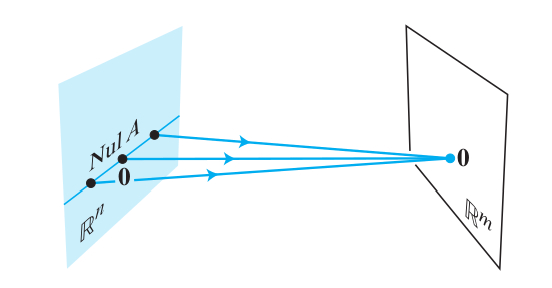
\includegraphics[width=0.3\textwidth]{figures/null_space.png}
    }}
    \end{center}

    \begin{center}\setlength{\fboxsep}{10pt}\fcolorbox{green!20}{green!20}{\parbox{0.9\linewidth}{
        \begin{theorem}
        A \textbf{null space} of and \(m\times n\) matrix \(A\) is a subspace of \(\mathbb{R}^n\). Equivalently, the set of all solutions of the homogeneous system \(A\mathbf{x}=\mathbf{0}\) is also a subspace of \(\mathbb{R}^n\).
        \end{theorem}
    }}
    \end{center}
    }
    \only<2>{
    \begin{center}\setlength{\fboxsep}{10pt}\fcolorbox{blue!20}{blue!20}{\parbox{0.9\linewidth}{
        \begin{definition}[Column Space]
            A \textbf{column space} or \textbf{range space} of matrix \(A\) is the set, \(Col A = Span(\{\text{Columns of } A\})\).  That is, the set of all linear combinations of the columns of \(A\).
        \end{definition}
    }}
    \end{center}

    \begin{center}\setlength{\fboxsep}{10pt}\fcolorbox{green!20}{green!20}{\parbox{0.9\linewidth}{
        \begin{theorem}
        The \textbf{column space} of an \(m\times n\) matrix \(A\) is a subspace of \(\mathbb{R}^m\). Equivalently, the set of all \(\mathbf{b}\in\mathbb{R}^m\) such that \(A\mathbf{x}=\mathbf{b}\) is the column space or range space (the range of the linear transformation \(A\mathbf{x}\)).
        \end{theorem}
    }}
    \end{center}
    }
    \only<3>{
    \textbf{Example 1:} Find the null space, (Nul\(A\)) of the matrix below
    \[
    A = \begin{bmatrix}
        \;\;\;1 & \;\;\;2 & -4 & 3 & -1\\
        -3 & -2 & \;\;\;1 & 0 & -1\\
        \;\;\;2 & -5 & \;\;\;1 & 8 & -3
    \end{bmatrix}
    \]
    
    \textbf{Example 2:} Find the null space, (Nul\(A\)) of the matrix below
    \[
    B = \begin{bmatrix}
        1 & -3 & \;\;\;5 & 0\\
        1 & \;\;\;2 & -1 & 0\\
        0 & \;\;\;7 & \;\;\;0 & 1 \\
        0 & \;\;\;0 & \;\;\;2 &  1
    \end{bmatrix}
    \]
    }
    \only<4>{
    \begin{center}\setlength{\fboxsep}{10pt}\fcolorbox{blue!20}{blue!20}{\parbox{0.9\linewidth}{
    \begin{definition}[Linear Transformation]
        A transformation \( T \) from \( \mathbb{R}^n \) to \( \mathbb{R}^m \) is linear if it satisfies the following:
        
        For any input vector \( \mathbf{u}, \mathbf{v} \in \mathbb{R}^n \) and scalar \(c\in\mathbb{R}\),
        \begin{enumerate}[(i)]
            \item \textbf{Additivity}: \( T(\mathbf{u} + \mathbf{v}) = T(\mathbf{u}) + T(\mathbf{v}) \).
            \item \textbf{Scalar Multiplication}: \( T(c\mathbf{u}) = cT(\mathbf{u}) \), for any scalar \( c \).
        \end{enumerate}
        
    \end{definition}
    }}
    \end{center}
    }
    \only<5>{
    \textbf{Example 1:} Find the column/range space, (Col\(A\)) of the matrix below
    \[
    A = \begin{bmatrix}
        \;\;\;1 & \;\;\;2 & -4 & 3 & -1\\
        -3 & -2 & \;\;\;1 & 0 & -1\\
        \;\;\;2 & -5 & \;\;\;1 & 8 & -3
    \end{bmatrix}
    \]

    \textbf{Example 2:} Find the column/range space, (Col\(A\)) of the matrix below
    \[
    B = \begin{bmatrix}
        1 & -3 & \;\;\;5 & 0\\
        1 & \;\;\;2 & -1 & 0\\
        0 & \;\;\;7 & \;\;\;0 & 1 \\
        0 & \;\;\;0 & \;\;\;2 &  1
    \end{bmatrix}
    \]
    }
\end{frame}


\begin{frame}{Contrast between Range/Column space and Null space/Kernel of an \(m\times n\) matrix, \(A\)}
\begin{columns}
    \begin{column}{0.5\textwidth}
        \begin{enumerate}
            \item Nul\(A\) is a subspace of \(\mathbb{R}^n\)
            \item Nul\(A\) is the solution to \(A\mathbf{x}=\mathbf{0}\). You have to find \(\mathbf{x}\) in order to find the null space.
            \item There is no obvious relation between Nul\(A\) and the columns or row of \(A\).
            \item Any vector \(\mathbf{v}\) is in the null space of \(A\) if and only if \(A\mathbf{v}=\mathbf{0}\).
            \item Nul \(A=\{\mathbf{0}\}\) if and only if the only solution to \(A\mathbf{x}=\mathbf{0}\) is the zero vector.
        \end{enumerate}
    \end{column}
    \begin{column}{0.5\textwidth}
        \begin{enumerate}
            \item Col\(A\) is a subspace of \(\mathbb{R}^m\)
            \item Col\(A\) is a linear combination of some of the columns of \(A\). \textbf{Select the columns that have pivots after row reduction}.
            \item The column vectors of \(A\) are in Col\(A\).
            \item Any vector \(\mathbf{b}\) is in the columns space of \(A\) if and only if \(A\mathbf{x}=\mathbf{b}\) is a consistent system. (You need to row reduce).
            \item Col \(A=\mathbb{R}^m\) if and only if \(A\mathbf{x}=\mathbf{b}\) has a pivot in each row.
        \end{enumerate}
    \end{column}
\end{columns}
\end{frame}


\subsection{Linearly Independent Sets and Bases}
\begin{frame}{Linearly Independent Sets and Bases}
\begin{center}\setlength{\fboxsep}{10pt}\fcolorbox{blue!20}{blue!20}{\parbox{0.9\linewidth}{
    \begin{definition}[Linear Independence]
        A set of vectors \( \{ \mathbf{v}_1, \mathbf{v}_2, \dots, \mathbf{v}_n \} \) in a vector space \( V \) is said to be \textbf{\textit{linearly independent}} if the only scalars \( c_1, c_2, \dots, c_n \) that satisfy:
        \[
        c_1 \mathbf{v}_1 + c_2 \mathbf{v}_2 + \cdots + c_n \mathbf{v}_n = \mathbf{0}
        \]
        are \( c_1 = c_2 = \cdots = c_n = 0 \).

        In other words, the solution to the homogeneous solution \(A\mathbf{x}=\mathbf{0}\) is the trivial solution.
    \end{definition}
}}\end{center} 

\end{frame}

\begin{frame}{Basis}
    \begin{center}\setlength{\fboxsep}{10pt}\fcolorbox{blue!20}{blue!20}{\parbox{0.9\linewidth}{
    \begin{definition}[Basis]
        Let \( H \) be a subspace of a vector space \( V \). A set \(\mathcal{B} =\{ \mathbf{b}_1, \mathbf{b}_2, \dots, \mathbf{b}_p \} \) is a basis in \(V\) for \(H\) if 
        \begin{enumerate}[(i)]
            \item \(\mathcal{B}\) is a linearly independent set
            \item \(Span(\mathcal{B})=H\)
        \end{enumerate}
    \end{definition}
    }}\end{center} 


    \begin{center}\setlength{\fboxsep}{10pt}\fcolorbox{blue!20}{blue!20}{\parbox{0.9\linewidth}{
    \begin{theorem}[The Basis Theorem]
        Let \( V \) be an \(n\)-dimensional vector space \( V \). Any linearly independent set \(\mathcal{L} =\{ \mathbf{v}_1, \mathbf{v}_2, \dots, \mathbf{v}_n \} \) is a basis for \(V\).

        That is, any linearly independent set with exactly \(n\) elements is a basis.
    \end{theorem}
}}\end{center} 
\end{frame}

\begin{frame}{Examples}
    \textbf{Example 1:} Find the basis of Col\(A\) and Nul\(A\) of the matrix below
    \[
    A = \begin{bmatrix}
        \;\;\;1 & \;\;\;2 & -4 & 3 & -1\\
        -3 & -2 & \;\;\;1 & 0 & -1\\
        \;\;\;2 & -5 & \;\;\;1 & 8 & -3\\
        -1 & \;\;\; 0 & \;\;\; 3 & 1 & \;\;\; 0
    \end{bmatrix}
    \]

    \textbf{Example 2:} Find the basis of Col\(A\) and Nul\(A\) of the matrix below
    \[
    B = \begin{bmatrix}
        1 & -3 & \;\;\;5 & 0\\
        1 & \;\;\;2 & -1 & 0\\
        0 & \;\;\;7 & \;\;\;0 & 1 \\
        0 & \;\;\;0 & \;\;\;2 &  1
    \end{bmatrix}
    \]

    \textbf{Example 3:} Are
    \(
    \mathcal{B} = \left\{
    \begin{bmatrix} \;\;\;1\\\;\;\;0\\-3 \end{bmatrix},
    \begin{bmatrix} 5\\1\\0 \end{bmatrix},
    \begin{bmatrix} -2\\\;\;\;0\\\;\;\;7 \end{bmatrix}
    \right\}
    \)
    and 
    \(
    \mathcal{D} = \left\{
    \begin{bmatrix} \;\;\;3\\\;\;\;2\\-4 \end{bmatrix},
    \begin{bmatrix} -2\\\;\;\;1\\\;\;\;0 \end{bmatrix}
    \begin{bmatrix} 3\\0\\1 \end{bmatrix},
    \begin{bmatrix} \;\;\;0\\\;\;\;2\\-3 \end{bmatrix}
    \right\}
    \)
    bases?
    \end{frame}




\subsection{Coordinate Systems}
\begin{frame}{Coordinate Systems}
    \begin{center}\setlength{\fboxsep}{10pt}\fcolorbox{green!20}{green!20}{\parbox{0.9\linewidth}{
    \begin{theorem}[Unique Representation]
        Let  \(\mathcal{B}=\{\mathbf{b}_1, \ldots,\mathbf{b}_p\}\) be a basis for a vector space \( V \).
        Then for each \(\mathbf{x} \in V\), there exists a unique set of scalars \(c_1, c_2,\ldots,c_p\) such that \(c_1\mathbf{b}_1 + c_2\mathbf{b}_2 + \cdots + c_p\mathbf{b}_p = \mathbf{x}\).
    \end{theorem}
    The \textbf{basis} imposes a coordinate system for that vector space.

    }}\end{center} 

    \begin{center}\setlength{\fboxsep}{10pt}\fcolorbox{blue!20}{blue!20}{\parbox{0.9\linewidth}{
    \begin{definition}[Basis]
        Let  \(\mathcal{B}=\{\mathbf{b}_1, \ldots,\mathbf{b}_p\}\) be a basis for a vector space \( V \).
        \textit{The coordinates of} \(\mathbf{x}\) \textit{relative to the basis} \(\mathcal{B}\)(or the \(\mathcal{B}-\)coordinates of \(\mathbf{x}\)) are a unique set of scalars \(c_1, c_2,\ldots,c_p\) such that \(c_1\mathbf{b}_1 + c_2\mathbf{b}_2 + \cdots + c_p\mathbf{b}_p = \mathbf{x}\).
    \end{definition}

    If \(c_1, c_2,\ldots,c_n\) are the \(\mathcal{B}-\)coordinates of \(\mathbf{x} \in \mathbb{R}^n\),
    \(
    [\mathbf{x}]_{\mathcal{B}}=\begin{bmatrix} c_1\\ \vdots\\c_n\end{bmatrix}
    \)
    is the \(\mathcal{B}-\)coordinate vector of \(\mathbf{x}\).
    }}\end{center} 
\end{frame}

\begin{frame}{Examples}
    \textbf{Example 1:}
    Let a basis \(\mathcal{B}=\left\{\begin{bmatrix} -1\\\;\;\;3\end{bmatrix},
    \begin{bmatrix} \;\;\;0\\ -2\end{bmatrix}\right\}\).
    Suppose that \(\mathbf{x}\in\mathbb{R}^2\) has the coordinate vector
    \([\mathbf{x}]_{\mathcal{B}}=\begin{bmatrix} -2\\ \;\;\;3\end{bmatrix}\).
    Find \(\mathbf{x}\).

    \textbf{Example 2:}
    Find the coordinate vector \([\mathbf{x}]_{\mathcal{B}}\) of \(\mathbf{x}\) from example 1 relative to the \textbf{standard basis} \(\mathcal{D}=\left\{\begin{bmatrix} 1\\0\end{bmatrix},
    \begin{bmatrix} 0\\ 1\end{bmatrix}\right\}\).

    \textbf{Example 3:}
    Let a basis \(\mathcal{B}=\left\{\begin{bmatrix} -1\\\;\;\;3\\ \;\;\;0\end{bmatrix},
    \begin{bmatrix} \;\;\;0\\ -2\\ \;\;\;5\end{bmatrix}\right\}\).
    \(H=Span(\mathcal{B})\) is a subspace.
    Determine whether \(\mathbf{x}=\begin{bmatrix} -3\\\;\;\;3\\\;\;\;15\end{bmatrix}\) is in the subspace \(H\), and find it's coordinate vector \([\mathbf{x}]_{\mathcal{B}}\).
\end{frame}

% We won't cover this
% \subsection{The Dimension of a Vector Space and Rank}
% \begin{frame}{The Dimension of a Vector Space and Rank}
    
% \end{frame}


\subsection{Change of Basis}
\begin{frame}{Change of Basis}
A \textbf{change of basis} allows us to represent vectors and linear transformations with respect to any coordinate systems of our choice.
\begin{center}\setlength{\fboxsep}{10pt}\fcolorbox{blue!20}{blue!20}{\parbox{0.9\linewidth}{
\begin{definition}[Change of Basis]
    Let \( \mathcal{B} = \{ \mathbf{b}_1, \mathbf{b}_2, \dots, \mathbf{b}_n \} \) and \( \mathcal{C} = \{ \mathbf{c}_1, \mathbf{c}_2, \dots, \mathbf{c}_n \} \) be two different bases of an \( n \)-dimensional vector space \( V \).
    
    Let \( [\mathbf{v}]_B \) and \( [\mathbf{v}]_C \) represent the \(\mathcal{B}\) - coordinate and \(\mathcal{C}\) - coordinate of the vector \(\mathbf{v} \) in bases \( \mathcal{B} \) and \(\mathcal{C}\) respectively, then its coordinate change form \([\mathbf{v}]_{\mathcal{B}}\) and  \( [\mathbf{v}]_{\mathcal{C}}\) is defined as:
    
    \[
    [\mathbf{v}]_{\mathcal{C}} = P_{\mathcal{B} \to \mathcal{C}} [\mathbf{v}]_{\mathcal{B}}
    \]
    
    where \( P_{\mathcal{B} \to \mathcal{C}} \) is the \textbf{change of basis matrix} from basis \(\mathcal{B}\) to basis \(\mathcal{C}\)
\end{definition}
}}
\end{center}
\end{frame}


\begin{frame}{Finding the Change of Basis Matrix}
The matrix \( P_{\mathcal{B}\to \mathcal{C}} \) is found by expressing each vector in \(\mathcal{B}\) in terms of the basis \(\mathcal{C}\).
\begin{eqnarray*}
\text{If }\quad\mathbf{b}_i = a_{1i} \mathbf{c}_1 + a_{2i} \mathbf{c}_2 + \dots + a_{ni} \mathbf{c}_n, &\text{ then } [\mathbf{b}_i]_{\mathcal{C}} =
\begin{bmatrix} a_{1i}\\ a_{2i}\\ \vdots\\ a_{ni} \end{bmatrix}
\\
\text{and }\;P_{\mathcal{B}\to \mathcal{C}}\; \text{ has columns }\;\; P_{\mathcal{B}\to \mathcal{C}} =& \begin{bmatrix} | & | & & | \\ [\mathbf{b}_1]_{\mathcal{C}} & [\mathbf{b}_2]_{\mathcal{C}} & \dots & [\mathbf{b}_n]_{\mathcal{C}} \\ | & | & & | \end{bmatrix}.
\end{eqnarray*}

Alternatively, if we know \( P_{\mathcal{C}\to \mathcal{B}} \), then
\[
P_{\mathcal{B}\to \mathcal{C}} = P_{\mathcal{C}\to \mathcal{B}}^{-1}.
\]
\end{frame}





\begin{frame}{Examples}
\only<1>{
\textbf{Example 1:}
Let \( {\mathcal{B}} = \left\{ \begin{bmatrix} 1 \\ 1 \end{bmatrix}, \begin{bmatrix} 2 \\ 3 \end{bmatrix} \right\} \) be a basis for \( \mathbb{R}^2 \). Express the vector \( \mathbf{v} = \begin{bmatrix} 5 \\ 7 \end{bmatrix} \) in the \( {\mathcal{B}} \)-basis.

\textbf{Solution:} 
Find scalars \( c_1, c_2 \) such that  
\[
\mathbf{v} = c_1 \begin{bmatrix} 1 \\ 1 \end{bmatrix} + c_2 \begin{bmatrix} 2 \\ 3 \end{bmatrix}.
\]

This gives the system:  
\[
\begin{cases}
c_1 + 2c_2 = 5, \\
c_1 + 3c_2 = 7.
\end{cases}
\;\;\Rightarrow\;\;
\begin{bmatrix}1 & 2\\ 1 & 3\end{bmatrix}\begin{bmatrix}c_1\\c_2\end{bmatrix} = \begin{bmatrix}5\\7\end{bmatrix}
\;\;\Rightarrow \;\;\;
\begin{bmatrix}1 & 2 & | & 5\\ 1 & 3 & | & 7\end{bmatrix}
\]

Solving, we get \( c_1 = 1 \), \( c_2 = 2 \), so \(
[\mathbf{v}]_{\mathcal{B}} = \begin{bmatrix} 1 \\ 2 \end{bmatrix}_{\mathcal{B}}.
\)
}

\only<2>{
    \textbf{Example 2:}
    Let  
    \(
    {\mathcal{B}} = \left\{ \begin{bmatrix} 1 \\ 2 \end{bmatrix}, \begin{bmatrix} 3 \\ 5 \end{bmatrix} \right\},\;
    {\mathcal{C}} = \left\{ \begin{bmatrix} 2 \\ 1 \end{bmatrix}, \begin{bmatrix} 4 \\ 3 \end{bmatrix} \right\}
    \)
    find the \textbf{change of basis matrix} \( P_{{\mathcal{B}} \to {\mathcal{C}}} \).
    
    \textbf{Solution:}  
    Express each vector in \( {\mathcal{B}} \) in terms of \( {\mathcal{C}} \):
    \begin{eqnarray*}
    \begin{bmatrix} 1 \\ 2 \end{bmatrix} = a_1 \begin{bmatrix} 2 \\ 1 \end{bmatrix} + a_2 \begin{bmatrix} 4 \\ 3 \end{bmatrix} \;\Rightarrow&\;
    \begin{bmatrix} 1 \\ 2 \end{bmatrix} = \begin{bmatrix} 2  & 4 \\ 1 & 3\end{bmatrix}
    \begin{bmatrix} a_1 \\ a_2 \end{bmatrix}\;\;\Rightarrow&\;\;
     \begin{bmatrix} 2 & 4 & | & 1\\ 1 & 3 & | & 2\end{bmatrix}, \text{ solve for } a_1 \text{ and } a_2\\
    \begin{bmatrix} 3 \\ 5 \end{bmatrix} = b_1 \begin{bmatrix} 2 \\ 1 \end{bmatrix} + b_2 \begin{bmatrix} 4 \\ 3 \end{bmatrix} \;\Rightarrow&\;
    \begin{bmatrix} 3 \\ 5 \end{bmatrix} = \begin{bmatrix} 2 & 4 \\ 1 & 3\end{bmatrix}
    \begin{bmatrix} b_1 \\ b_2 \end{bmatrix}\;\;\Rightarrow&\;\;
    \begin{bmatrix} 2 & 4 & | & 3\\ 1 & 3 & | & 5\end{bmatrix}, \text{ solve for } b_1 \text{ and } b_2.
    \end{eqnarray*}
    
    Solving both systems, we get 
    \(\begin{bmatrix} a_1 \\ a_2 \end{bmatrix} =  \begin{bmatrix} -\frac{5}{2}\\\;\;\;\frac{3}{2} \end{bmatrix}\)
    and 
    \(\begin{bmatrix} b_1 \\ b_2 \end{bmatrix} = \begin{bmatrix} -\frac{11}{2}\\\;\;\;\frac{7}{2} \end{bmatrix}\).
    So,
    \(
    P_{{\mathcal{B}} \to {\mathcal{C}}} =
    \begin{bmatrix}
    -\frac{5}{2} & -\frac{11}{2} \\
    \;\;\;\frac{3}{2} & \;\;\;\frac{7}{2}
    \end{bmatrix}.
    \)
    
    \textbf{Alternatively,} solve
    \[
    \begin{bmatrix} 2 & 4 & | & 1 & 3\\ 1 & 3 & | & 2 & 5\end{bmatrix}
    \;\;\; \to \;\;\;
    \begin{bmatrix} 1 & 0 & | & -\frac{5}{2} & -\frac{11}{2}\\ 0 & 1 & | & \;\;\;\frac{3}{2} & \;\;\;\frac{7}{2}\end{bmatrix}
    \]
}
\only<3>{
\textbf{Try your hands on the following problems:}
\begin{enumerate}
    \item  Given \( {\mathcal{B}} = \{ \mathbf{b}_1, \mathbf{b}_2 \} \) and \( {\mathcal{C}} = \{ \mathbf{c}_1, \mathbf{c}_2 \} \), describe the steps to compute the change of basis matrix \( P_{{\mathcal{B}} \to {\mathcal{C}}} \).
    \item If the transformation matrix of \( T \) in the standard basis is:
    \[
    A = \begin{bmatrix} 4 & 2 \\ 3 & 1 \end{bmatrix},
    \]
    what is its representation in a new basis \( {\mathcal{B}} \) with basis vectors \( \mathbf{b}_1 = (3,1) \) and \( \mathbf{b}_2 = (2,-1) \)?

    \textbf{Hint:} to get the representation of \(T\) in the basis \(\mathcal{B}\), you 
 need to \emph{\textcolor{red}{transform your vector from the \(\mathcal{B}\)-coordinate to the standard coordinate system \(\mathcal{E}\)}, \textcolor{cyan}{then apply the transformation}, and \textcolor{blue}{then return the vector back to the \(\mathcal{B}\)-coordinate system}.} Now multiply all 3 in that order to get the new transformation matrix in the \(\mathcal{B}\)-coordinate system.
    
    \item Let \( {\mathcal{B}} = \{ (2,1), (1,3) \} \) and \( {\mathcal{C}} = \{ (3,2), (4,1) \} \).
    Find the matrix \( P_{{\mathcal{B}} \to {\mathcal{C}}} \).
\end{enumerate}
}
\end{frame}


\begin{frame}{Homework 10}
\textbf{Question 1: }
Let \( {\mathcal{B}} = \left\{ \mathbf{b}_1, \mathbf{b}_2, \mathbf{b}_3 \right\} \) be the basis: 
\(
\mathbf{b}_1 = \begin{bmatrix} 1 \\ 0 \\ 1 \end{bmatrix}, \quad
\mathbf{b}_2 = \begin{bmatrix} 0 \\ 1 \\ 1 \end{bmatrix}, \quad
\mathbf{b}_3 = \begin{bmatrix} 1 \\ 1 \\ 0 \end{bmatrix}.
\)
Express the vector \( \mathbf{v} = \begin{bmatrix} 3 \\ 4 \\ 5 \end{bmatrix} \) in the \( {\mathcal{B}} \)-basis.

\vspace{.25cm}

\textbf{Question 2:}
Let:
\(
{\mathcal{B}} = \left\{ \begin{bmatrix} 1 \\ 2 \\ 1 \end{bmatrix}, \begin{bmatrix} 0 \\ 1 \\ 2 \end{bmatrix}, \begin{bmatrix} 2 \\ 0 \\ 3 \end{bmatrix} \right\}, \quad
{\mathcal{C}} = \left\{ \begin{bmatrix} 2 \\ 1 \\ 1 \end{bmatrix}, \begin{bmatrix} 1 \\ 3 \\ 4 \end{bmatrix}, \begin{bmatrix} 0 \\ 1 \\ 1 \end{bmatrix} \right\}.
\)
Find the change of basis matrix \( P_{{\mathcal{B}} \to {\mathcal{C}}} \).

\vspace{.25cm}

\textbf{Question 3:}
If the transformation matrix of \( T \) in the basis \( {\mathcal{H}} \) with basis vectors \( \mathbf{h}_1 = (3,1) \) and \( \mathbf{h}_2 = (0,1) \) is:
   \[
   A = \begin{bmatrix} 4 & 2 \\ 3 & 1 \end{bmatrix},
   \]
   what is its representation in a new basis \( {\mathcal{B}} \) with basis vectors \( \mathbf{b}_1 = (3,1) \) and \( \mathbf{b}_2 = (2,-1) \)?
\end{frame}


\section{Eigenvalues and Eigenvectors}
\subsection{Eigenvectors and Eigenvalues (and Complex Eigenvalues)}
\begin{frame}{Eigenvectors and Eigenvalues}
    \begin{center}\setlength{\fboxsep}{10pt}\fcolorbox{blue!20}{blue!20}{\parbox{0.9\linewidth}{
    \begin{definition}[Eigenvectors]
     Given a square matrix \( A \), a nonzero vector \(\mathbf{v}\) is an eigenvector of \( A \) if there exists a scalar \( \lambda \) such that:
    \[
    A\mathbf{v} = \lambda \mathbf{v}
    \]
    where \( \lambda \) is called the \textbf{eigenvalue} corresponding to \( \mathbf{v} \).
    \end{definition}
    }}
    \end{center}

    \textbf{Example 1:}
    Given the matrix \(A = \begin{bmatrix} 1 & 6\\ 5 & 2 \end{bmatrix}\), are 
    \(\mathbf{u}=\begin{bmatrix} \;\;\;6\\-5 \end{bmatrix}\) and 
     \(\mathbf{v}=\begin{bmatrix} \;\;\;3\\-2 \end{bmatrix}\) eigenvectors of \(A\)?

    \textbf{Example 2:}
    Given  \(B = \begin{bmatrix}4 & -1 & 6\\ 2 & \;\;\; 1 & 6\\ 2 & -1 & 8\end{bmatrix}\), are 
    \(\mathbf{u}=\begin{bmatrix} -3 \\ \;\;\;0 \\ \;\;\;1\end{bmatrix}\) and 
     \(\mathbf{v}=\begin{bmatrix} 1 \\ 2\\0 \end{bmatrix}\) eigenvectors of \(B\)?
\end{frame}


\begin{frame}{Computing Eigenvalues and Eigenvectors}
\only<1>{
\textbf{To find the eigenvalues of a matrix} \( A \), solve the characteristic equation:
\[
\det(A - \lambda I) = 0
\quad
\text{where } I \text{ is the identity matrix of the same dimension as } A.
\]


Once an eigenvalue \( \lambda \) is found, we obtain it's corresponding eigenvector \( \mathbf{v} \) by solving:
\[
(A - \lambda I) \mathbf{v} = 0
\]
for each eigenvalue \( \lambda \).
}
\only<2>{
\textbf{Example 1:}
Find the eigenvalues and eigenvectors for the matrix:
\(A = \begin{bmatrix} 4 & 2 \\ 1 & 3 \end{bmatrix}\)

\begin{enumerate}
    \item \textbf{Compute the Characteristic Equation}
    \(
    \det \left( \begin{bmatrix} 4 & 2 \\ 1 & 3 \end{bmatrix} - \lambda \begin{bmatrix} 1 & 0 \\ 0 & 1 \end{bmatrix} \right) = 0
    \)
    \[
    \det \left(\begin{bmatrix} 4 - \lambda & 2 \\ 1 & 3 - \lambda \end{bmatrix}\right) = 0
    \quad \Rightarrow \quad
    (4 - \lambda)(3 - \lambda) - (2)(1) = 0
    \]
    \[
    12 - 4\lambda - 3\lambda + \lambda^2 - 2 = 0
    \quad \Rightarrow \quad
    \lambda^2 - 7\lambda + 10 = 0 \quad \Rightarrow \quad \lambda = 5, 2
    \]

    \item \textbf{Finding the  Eigenvectors}
    
    for \( \lambda = 5 \),
    \[
    (A - 5I) \mathbf{v} = 0
   \quad \Rightarrow \quad
    \begin{bmatrix} -1 & 2 \\ 1 & -2 \end{bmatrix} \begin{bmatrix} x \\ y \end{bmatrix} = \begin{bmatrix} 0 \\ 0 \end{bmatrix}
    \quad \Rightarrow \quad 
    \mathbf{v_1} = \begin{bmatrix} 2 \\ 1 \end{bmatrix}.
    \]
    
    For \( \lambda = 2 \),
    \[
    (A - 2I) \mathbf{v} = 0
   \quad \Rightarrow \quad
    \begin{bmatrix} 2 & 2 \\ 1 & 1 \end{bmatrix} \begin{bmatrix} x \\ y \end{bmatrix} = \begin{bmatrix} 0 \\ 0 \end{bmatrix}
    \quad \Rightarrow \quad
    \mathbf{v_2} = \begin{bmatrix} -1 \\ 1 \end{bmatrix}.
    \]
\end{enumerate}
}

\only<3>{
\textbf{Example 2:}
Find its eigenvalues and eigenvectors for the matrix
\(\quad
B = \begin{bmatrix} 6 & -1 & 0 \\ -1 & 6 & -1 \\ 0 & -1 & 6 \end{bmatrix}
\)


\textbf{Compute the Characteristic Equation}
\( \;\;
\det(B - \lambda I) = \begin{vmatrix} 6 - \lambda & -1 & 0 \\ -1 & 6 - \lambda & -1 \\ 0 & -1 & 6 - \lambda \end{vmatrix} = 0
\)

\textbf{Ans:}
\(
\lambda_1 = 6,\; \mathbf{v_1}=\begin{bmatrix}-1\\ \;\;0\\ \;\;1\end{bmatrix};
\quad
\lambda_2 = 6-\sqrt{2},\; \mathbf{v_2}=\begin{bmatrix}1\\ \sqrt{2}\\1\end{bmatrix};
\quad
\lambda_3 = 6+\sqrt{2},\; \mathbf{v_3}=\begin{bmatrix} \;\;1\\ -\sqrt{2}\\\;\;1\end{bmatrix}
\)

\vspace{.5cm}

\textbf{Example 3:}
Find its eigenvalues and eigenvectors of
\(
D = \begin{bmatrix} 6 & -1 & 0 \\ -1 & 6 & -1 \\ 0 & 0 & 6 \end{bmatrix}
\)

\textbf{Ans:}
\(
\lambda_1 = 5,\; \mathbf{v_1}=\begin{bmatrix} 1\\1\\0 \end{bmatrix};
\quad
\lambda_2 =6,\; \mathbf{v_2}=\begin{bmatrix} -1\\\;\;0\\\;\;1 \end{bmatrix};
\quad
\lambda_3 =7,\; \mathbf{v_3}=\begin{bmatrix} -1\\\;\;1\\\;\;0 \end{bmatrix};
\)
}
\only<4>{
\textbf{Additional Practice Problems (Homework)}
\begin{enumerate}
    \item Find the eigenvalues and eigenvectors of
   \[
   C = \begin{bmatrix} 2 & -1 \\ -1 & 2 \end{bmatrix}
   \]
    \item Compute the eigenvalues and eigenvectors of the 3×3 matrix:
   \[
   D = \begin{bmatrix} -26 & -33 & -2 \\ 31 & 42 & 23 \\ -11 & -15 & -4 \end{bmatrix}
   \]
    \item Prove that the eigenvalues of an upper triangular matrix correspond to the values on the main diagonal.
    \item \textbf{Extra-if you want to try}: Show that if \(\mathbf{v}_1,\ldots,\mathbf{v}_n\) are eigenvectors that correspond to distinct eigenvalues \(\lambda_1,\ldots,\lambda_n\) of an \(n\times n\) matrix \(A\), then the set \(\{\mathbf{v}_1,\ldots,\mathbf{v}_n\}\) is linearly independent.
\end{enumerate}
}
\end{frame}


\begin{frame}{More on Eigenvectors and Eigenvalues}
    \begin{center}\setlength{\fboxsep}{10pt}\fcolorbox{green!20}{green!20}{\parbox{0.9\linewidth}{
    \begin{theorem}
     Let \( A \) be an \(n\times n\) matrix.
     Then \( A \) is invertible if and only if \(\lambda=0\) is \textbf{not} an eigenvalue of \(A\).
    \end{theorem}
    }}
    \end{center}

    \begin{center}\setlength{\fboxsep}{10pt}\fcolorbox{blue!20}{blue!20}{\parbox{0.9\linewidth}{
    \begin{definition}[Similarity]
     An \(n\times n\) matrix \( A \), is \textbf{similar} to an \(n\times n\) matrix \(B\) if there exists an invertible matrix \(P\) such that \( P^{-1}AP = B \).
    \end{definition}
    }}
    \end{center}

    If \(A\) and \(B\) are \textbf{similar}, then they have the same characteristic polynomial, and hence the same eigenvalues (with the same multiplicities.)
\end{frame}


\subsection{Diagonalization}
\begin{frame}{Diagonalization}
\only<1>{
    An \(n\times n\) matrix \( D  \) is \textbf{diagonal} if all its entries off the main diagonal are zero.
    
    \textbf{Diagonalization} is the process of converting a square matrix \( A \) into a diagonal matrix \( D \) by means of a \textit{similarity transformation}.
    
    \begin{center}\setlength{\fboxsep}{10pt}\fcolorbox{blue!20}{blue!20}{\parbox{0.9\linewidth}{
    \begin{definition}[Diagonalizability]
     A square matrix \( A \) is \textbf{diagonalizable} if there exists an invertible matrix \( P \) and a diagonal matrix \( D \) such that:

    \[
    A = P D P^{-1}
    \]
    where \( D \) is a diagonal matrix with eigenvalues of \( A \) on the diagonal.
    The columns of \( P \) are the eigenvectors of \( A \).

    In other words, \(A\) is similar to \(D\).
    \end{definition}
    }}
    \end{center}
    }
    \only<2>{
    \begin{center}\setlength{\fboxsep}{10pt}\fcolorbox{green!20}{green!20}{\parbox{0.9\linewidth}{
        \begin{theorem}[Conditions for Diagonalizability]
         An \( n \times n \) matrix, \( A \) is diagonalizable if and only if:
         \begin{enumerate}
             \item It has \( n \) linearly independent eigenvectors.
             \item The algebraic multiplicity of each eigenvalue equals its geometric multiplicity (If an eigenvalue has a multiplicity of \(2\), then that eigenvalue has \(2\) corresponding eigenvectors).
             \item It has eigenvectors \(\mathbf{v}_1, \mathbf{v}_2,\ldots,\mathbf{v}_n\) , and the matrix of eigenvectors \(P = \begin{bmatrix}\mathbf{v}_1 & \mathbf{v}_2 & \ldots & \mathbf{v}_n \end{bmatrix}\) is invertible.
         \end{enumerate}
        \end{theorem}
        }}
        \end{center}
    }   
    \only<3>{
    \begin{center}\setlength{\fboxsep}{10pt}\fcolorbox{red!20}{red!20}{\parbox{0.9\linewidth}{
        \begin{corollary}[Steps to Diagonalize a Matrix]
         To diagonalize a diagonalizable matrix, \( A \):
         \begin{enumerate}
             \item \textbf{Find the eigenvalues: } Solve \( \det(A - \lambda I) = 0 \).
             \item \textbf{Find the eigenvectors: } Solve \( (A - \lambda I)x = 0 \) for each eigenvalue \( \lambda \).
             \item \textbf{Check independence: } Ensure there are \( n \) linearly independent eigenvectors.
             \item \textbf{Form \( P \) and \( D \):}
             \begin{itemize}
                 \item \( P \) consists of the eigenvectors as column
                 \item \( D \) is a diagonal matrix with eigenvalues on the diagonal.
             \end{itemize}
            \item Compute \( P^{-1} A P \) to confirm \( D \) to \textbf{verify}.
         \end{enumerate}
        \end{corollary}
        }}
        \end{center}
    
    \textbf{Useful things to note:}
    \begin{itemize}
        \item Symmetric Matrices are always diagonalizable, and their eigenvectors are orthogonal (we will talk about this in the next module).
        \item Simplifies matrix exponentiation (\( A^n = P D^n P^{-1} \)).science.
    \end{itemize} 
    }
    \end{frame}
    \begin{frame}{Examples}
    \only<1>{
    \begin{center}\setlength{\fboxsep}{10pt}\fcolorbox{green!20}{green!20}{\parbox{0.9\linewidth}{
        \begin{theorem}[The Diagonalization Theorem]
         An \(n\times n\) matrix with \(n\) distinct eigenvalues is diagonalizable.
        \end{theorem}

        \textbf{NOTE:} this \textcolor{red}{does not} imply that, if a matrix \textcolor{red}{does not have } \(n\) \textcolor{red}{distinct eigenvalues, then it is not diagonalizable}.

        Check \textbf{Conditions for Diagonalizability Theorem}
        }}
    \end{center}
    
    \textbf{Example 1:}
    
    Diagonalize the matrix \(A = \begin{bmatrix}
        7 & 2\\ -4 & 1
    \end{bmatrix}\) if possible.
    And find a formula for \(A^k\), given that \(A = P D P^{-1}\).
    }
    \only<2>{ \textbf{Example 2:}
    
    Diagonalize the following matrix, if possible.
    \[
    A = \begin{bmatrix}
        2 & 0 &\;\; 0 \\ 1 & 2 & -1 \\ 1 & 3 & -2
    \end{bmatrix}.
    \]
    \begin{center}\setlength{\fboxsep}{10pt}\fcolorbox{yellow!20}{yellow!20}{\parbox{0.9\linewidth}{
    \textbf{Solution}
    
    The eigenvalues of \(A\) are \(\lambda_1=2,\, \lambda_2=1,\, \lambda_3=-1\).
    So by the diagonalization theorem, \(A\) is diagonalizable since it has \(3\) distinct eigenvalues.

    It has corresponding eigenvectors 
    \(\mathbf{v}_1=\begin{bmatrix} 1\\1\\1 \end{bmatrix},\,
    \mathbf{v}_2=\begin{bmatrix} 0\\1\\1 \end{bmatrix},\;
    \)
    and
    \(\mathbf{v}_3=\begin{bmatrix} 0\\1\\3 \end{bmatrix}\)
    respectively.

    So, \(P = \begin{bmatrix} 1&0&0\\1&1&1\\1&1&3 \end{bmatrix}\)
    and \(D = \begin{bmatrix} 2&0&0\\0&1&0\\0&0&-1 \end{bmatrix}\),
    
    where \(A = PDP^{-1}\).
    }}
    \end{center}
    }
    \only<3>{ \textbf{Example 3:}
    
    Diagonalize the matrix, \(
    A = \begin{bmatrix} 0&1&1 \\ 1&0&1 \\ 1&1& 0 \end{bmatrix}.
    \) if possible.
    \begin{center}\setlength{\fboxsep}{10pt}\fcolorbox{yellow!20}{yellow!20}{\parbox{0.9\linewidth}{
    \textbf{Solution}
    
    The eigenvalues of \(A\) are \(\lambda_1=2,\, \lambda_{2,3}=-1\).
    So the \textbf{diagonalization theorem} cannot guarantee that \(A\) is diagonalizable since it does not have \(3\) distinct eigenvalues.

    It has corresponding eigenvectors 
    \(\mathbf{v}_1=\begin{bmatrix} 1\\1\\1 \end{bmatrix},
    \)

    Continue the solution to see whether \(A\) is diagonalizable.
    If \(\lambda_{2,3}\) yields two eigenvectors, then it is. And you can go ahead to find the corresponding \(P\) and \(D\).
    }}
    \end{center}
    }
    \only<4>{
    \textbf{Example 4:}
    
    Diagonalize the following matrix, if possible.
    \[
    A = \begin{bmatrix}
        \;\;1 & \;\;3 &\;\; 3 \\ -3 & -5 & -3 \\ \;\;3 & \;\;3 & \;\;1
    \end{bmatrix}.
    \]
    That is, find an invertible matrix \(P\) and a diagonal matrix \(D\) such that \(A = P D P^{-1}\).
    
    
    \textbf{Example 5:}
    
    Determine whether \(A = \begin{bmatrix}
        5 & -8 &\;\; 1 \\ 0 & \;\;0 & \;\;7 \\ 0 & \;\;0 & -2
    \end{bmatrix}\) is diagonalizable.
    }
    \only<5>{
    \begin{center}\setlength{\fboxsep}{10pt}\fcolorbox{green!20}{green!20}{\parbox{0.9\linewidth}{
        \begin{theorem}
         Let \(A\) be an \(n\times n\) matrix whose distinct eigenvalues are  \(\lambda_1,\lambda_2,\ldots,\lambda_p\).
         \begin{enumerate}[a.]
             \item For \(1\leq k \leq p\), the dimension of the eigenspace for \(\lambda_k\) is less than or equal to the multiplicity of the eigenvalue \(\lambda_k\).
             \item The matrix \(A\) is diagonalizable if and only if the sum of the dimensions of the eigenspaces  equals \(n\), and this happens if and only if 
             \begin{itemize}
                 \item the characteristic polynomial factors completely into linear factors
                 \item the dimension of the eigenspace for each \(lambda_k\) equals the multiplicity of \(\lambda_k\)
             \end{itemize}
             \item If \(A\) is diagonalizable and \(\mathcal{B}_k\) is a basis for the eigenspace corresponding to \(\lambda_k\) for each \(k\), then the total collection of vectors in the set \(\mathcal{B}_1,\ldots,\mathcal{B}_p\) forms an eigenvector basis for \(\mathbb{R}^n\)
         \end{enumerate}
        \end{theorem}
        }}
        \end{center}
    }
    \only<6>{
    Diagonalize the following matrices if possible
    \begin{enumerate}[a)]
        \item \(A = \begin{bmatrix}
        1 & \;\;0 \\ 6 & -1
        \end{bmatrix}\)
        \item \(A = \begin{bmatrix}
        2 & 3 \\ 4 & 1
        \end{bmatrix}\)
        \item \(A = \begin{bmatrix}
        \;\;2 & \;\;2 & -1 \\ \;\;1 & \;\;3 & -1 \\ -1 & -2 & \;\;2
        \end{bmatrix}\)
        \item \(A = \begin{bmatrix}
        4 & 0 & 0 & 0 \\ 0 & 4 & 0 & 0 \\ 0 & 0 & 2 & 0\\1 & 0 & 0&2
    \end{bmatrix}\)
    \item \(A = \begin{bmatrix}
        -6 & \;\;4 & 0 & 9 \\ -3 & \;\;0 & 1 & 6 \\
        -1 & -2 & 1 & 0 \\ -4 & \;\;4 & 0 & 7
    \end{bmatrix}\)
    \end{enumerate}
    }
\end{frame}

\begin{frame}{Homework 11}

\begin{enumerate}
    \item Determine whether the following are diagonalizable: If so, diagonalize them.
    \begin{enumerate}[a)]
        \item \[A_1 =\begin{bmatrix} 1 & 1\\ 0 & 1 \end{bmatrix}\]

        \item \[ A_2 = \begin{bmatrix}
            \;\;1 & \;\;3 &\;\; 3 \\
            -3 & -5 & -3 \\
            \;\;3 & \;\;3 & \;\;1
            \end{bmatrix}.\]
    
        \item \[A_3 = \begin{bmatrix}
            5 & -8 &\;\; 1 \\
            0 & -3 & \;\;7 \\
            0 & \;\;0 & -2
    \end{bmatrix}.\] 
    \end{enumerate}
    \item Determine whether
    \(A =\begin{bmatrix} 2 & 1\\ 0 & 2 \end{bmatrix}\) and 
    \(B =\begin{bmatrix} 2 & 0\\ 0 & 2 \end{bmatrix}\) are similar.
\end{enumerate}
\end{frame}


% \subsection{Eigenvectors and Linear Transformations}
% \begin{frame}{Eigenvectors and Linear Transformations}
    
% \end{frame}

\begin{frame}{Complex Eigenvalues}
    \begin{enumerate}
        \item Find the eigenvalues and corresponding eigenvectors of \(A = \begin{bmatrix}
        0 & -1 \\ 1 & \;\;0
        \end{bmatrix}\)

        \item  Find the eigenvalues and corresponding eigenvectors \[A = \begin{bmatrix}
        \frac{1}{2} & -\frac{3}{5} \\ \frac{3}{4} & \;\;\frac{11}{10}
        \end{bmatrix}\]
    \end{enumerate}
\end{frame}



\section{Orthogonality and Least Squares}
\subsection{Inner Product, Length, and Orthogonality}
\begin{frame}{Inner Product, Length, and Orthogonality}
\only<1>{
The \textbf{inner product}  provides \textit{a way to measure the similarity between two vectors}.

\begin{center}\setlength{\fboxsep}{10pt}\fcolorbox{blue!20}{blue!20}{\parbox{0.9\linewidth}{
        \begin{definition}{Inner Product}
        For vectors \( \mathbf{u}, \mathbf{v} \in \mathbb{R}^n \), the inner product (or dot product) is:
        \[
        \mathbf{u} \cdot \mathbf{v} = \mathbf{u}^{\top} \mathbf{v}
        = \begin{bmatrix} u_1 & u_2 & \dots & u_n \end{bmatrix}\begin{bmatrix} v_1 \\ v_2 \\ \dots \\ v_n \end{bmatrix}
        = u_1 v_1 + u_2 v_2 + \dots + u_n v_n.
        \]
        \end{definition}
    }}
\end{center}
}
\only<2>{
\begin{center}\setlength{\fboxsep}{10pt}\fcolorbox{green!20}{green!20}{\parbox{0.9\linewidth}{
        \begin{theorem}{Properties of Inner Product}
        For  all vectors \( \mathbf{u}, \mathbf{v}, \mathbf{w} \in \mathbb{R}^n\) and scalar \( c \):
        \begin{enumerate}[a)]
        \item \( \mathbf{u} \cdot \mathbf{v} \in \mathbb{R} \).
        \item \textbf{Commutativity:} \( \mathbf{u} \cdot \mathbf{v} = \mathbf{v} \cdot \mathbf{u} \)
        \item \textbf{Distributivity:} \( \mathbf{u} \cdot (\mathbf{v} + \mathbf{w}) = \mathbf{u} \cdot \mathbf{v} + \mathbf{u} \cdot \mathbf{w} \)
        \item \textbf{Scalar Multiplication:} \( (c\mathbf{u}) \cdot \mathbf{v} = c(\mathbf{u} \cdot \mathbf{v}) \)
        \item \textbf{Non-Negativity:} \( \mathbf{u} \cdot \mathbf{u} \geq 0 \), with equality only if \( \mathbf{u} = 0 \).
        \end{enumerate}
        \end{theorem}
    }}
\end{center}
}


\only<3>{
\begin{center}\setlength{\fboxsep}{10pt}\fcolorbox{blue!20}{blue!20}{\parbox{0.9\linewidth}{
        \begin{definition}{Length (Norm) of a Vector}
        The \textbf{length} (or \textbf{norm}) of a vector \( \mathbf{v} \) in \( \mathbb{R}^n \) is given by:

        \[
        \|\mathbf{v}\| = \sqrt{\mathbf{v} \cdot \mathbf{v}} = \sqrt{v_1^2 + v_2^2 + \dots + v_n^2}
        \]

        The \textbf{length} or \textbf{distance} between two vectors \(\mathbf{u}\) and \(\mathbf{v}\) is the \textbf{length} of difference vector.
        That is,
        \[\|u-v\|\]
        
        \end{definition}
    }}
\end{center}
}
\only<4>{
\textbf{Example 1:} Find the distance be the vectors \(\mathbf{u}_1 =\begin{bmatrix} 1 \\ 6 \end{bmatrix}\) and 
\(\mathbf{u}_2 =\begin{bmatrix} \;\;0 \\ -2 \end{bmatrix}\)

\vspace{0.25cm}

\textbf{Example 2:} Find the length of  the vector \(\mathbf{v} =\begin{bmatrix} -3 \\ 1 \\ 6 \end{bmatrix}\).

\vspace{0.25cm}

\textbf{Example 3:} Find the inner product between the vectors \(\mathbf{u}_1 =\begin{bmatrix} 3 \\ 2 \\ 0 \end{bmatrix}\) and 
\(\mathbf{u}_2 =\begin{bmatrix} \;\;7\\ \;\;0 \\ -2 \end{bmatrix}\)
}

\only<5>{
\begin{center}\setlength{\fboxsep}{10pt}\fcolorbox{blue!20}{blue!20}{\parbox{0.9\linewidth}{
        \begin{definition}{Orthogonal Vectors}
Two vectors \( \mathbf{u}, \mathbf{v} \) are \textbf{orthogonal} (perpendicular) if their inner product is zero:

\[
\mathbf{u} \cdot \mathbf{v} = 0
\]
\end{definition}
}}
\end{center}

\textbf{Example 4:} Prove that 
\(\|\mathbf{u} + \mathbf{v} \|^2 = \| \mathbf{u}\|^2 + \| \mathbf{v}\|^2\) if the vectors \(\mathbf{u}\) and \(\mathbf{v}\) are \textbf{orthogonal}.

\vspace{0.25cm}

\textbf{Example 5:} Prove that 
\((\|\mathbf{u}\| + \|\mathbf{v} \|)^2 \geq \| \mathbf{u}\|^2 + \| \mathbf{v}\|^2\) for all the vectors \(\mathbf{u}\) and \(\mathbf{v}\).

\vspace{0.25cm}

\textbf{Example 6:} Prove that 
\(\|c\mathbf{v}\| = |c|\|\mathbf{v}\|\) for all the vectors \(\mathbf{v}\).
}
\only<6>{
    \begin{center}\setlength{\fboxsep}{10pt}\fcolorbox{blue!20}{blue!20}{\parbox{0.9\linewidth}{
        \begin{definition}{Relations between Inner Product and Angles}
    The inner product of two vectors \( \mathbf{u}, \mathbf{v} \) can also be expressed in terms of their direction as:
    
    \[
    \mathbf{u} \cdot \mathbf{v} = \|\mathbf{u}\|\|\mathbf{v}\|\cos{\theta}
    \]
    where \(\theta\) is the angle between the two vectors.
    \end{definition}
    }}
    \end{center}
    }
\end{frame}

\subsection{Orthogonal Sets}
\begin{frame}{Orthogonal Sets}
A set of vectors \(\{\mathbf{v}_1, \mathbf{v}_2, \ldots,\mathbf{v}_n \}\) is \textbf{orthogonal} if each pair of distinct vectors within the set \(\mathbf{v}_i\) and \(\mathbf{v}_j\) are \textbf{orthogonal}.
That is, \(\mathbf{v}_i\cdot \mathbf{v}_j=0\)

\vspace{0.25cm}

\textbf{Example 1:} Show that the set of vectors \(\{\mathbf{v}_1, \mathbf{v}_2, \mathbf{v}_3\}\) are orthogonal.
\[\mathbf{v}_1 =\begin{bmatrix} 3\\1 \\ 1 \end{bmatrix}, \,\mathbf{v}_2 =\begin{bmatrix} -\frac{1}{2}\\-2 \\ \;\;\frac{7}{2} \end{bmatrix},\, \text{ and } 
\mathbf{v}_3 =\begin{bmatrix} -1\\\;\;2 \\ \;\;0 \end{bmatrix}\]

\vspace{0.25cm}

\textbf{Example 2:} Are the following  vectors, \(\mathbf{u}_1 =\begin{bmatrix} 1 \\ 6 \end{bmatrix}\) and 
\(\mathbf{u}_2 =\begin{bmatrix} \;\;0 \\-2 \end{bmatrix}\) orthogonal?

\vspace{0.3cm}

\textbf{Example 3:} Given that a set of nonzero vectors \(\{\mathbf{v}_1, \mathbf{v}_2, \mathbf{v}_3\}\) are orthogonal, show that the set is linearly independent.

\end{frame}

\begin{frame}{Orthogonal Projections}
Given a nonzero vector \(\mathbf{u}\in\mathbb{R}^n\), a different vector, \(\mathbf{y}\in\mathbb{R}^n\) can always decomposed into a two components; one, a multiple  of \(\mathbf{u}\) (parallel to \(\mathbf{u}\)), and the orthogonal to \(\mathbf{u}\).

The vector component of \(\mathbf{y}\) that is a multiple  of \(\mathbf{u}\) or parallel to \(\mathbf{u}\) is called the \textbf{Orthogonal Projection:} The projection of \( \mathbf{y} \) onto \(\mathbf{u}\) (if \( \mathbf{u} \neq 0 \)) is:

\begin{columns}
    \begin{column}{0.5\textwidth}
    \[
    \hat{\mathbf{y}} =\text{proj}_{\mathbf{u}} \mathbf{y} = \frac{\mathbf{y} \cdot \mathbf{u}}{\mathbf{u} \cdot \mathbf{u}} \mathbf{u}
    \]
    \hspace{0.7cm} The vector, \(\mathbf{y}\) can be written as a sum of 
    
    \hspace{0.7cm} \(\mathbf{u}\) and \(\text{proj}_{\mathbf{u}} \mathbf{y}\).
    \end{column}
    \begin{column}{0.6\textwidth}
    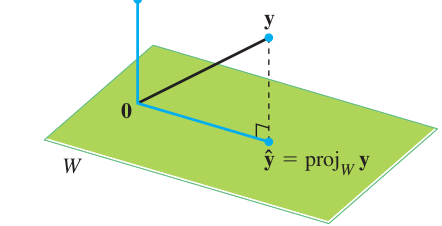
\includegraphics[width=0.6\textwidth]{figures/projection.png}
    \end{column}
\end{columns}


Alternatively if \(W=Span(\{\mathbf{u}_1,\mathbf{u}_2,\ldots,\mathbf{u}_n)\}\) where the \(\mathbf{u}_i\)'s are orthogonal, we say the \textbf{orthogonal projection} of \(\mathbf{y}\) onto the subspace spanned by \(W\) is
\[
\hat{\mathbf{y}} =\text{proj}_{\mathbf{u}} \mathbf{y} = \frac{\mathbf{y} \cdot \mathbf{u}_1}{\mathbf{u}_1 \cdot \mathbf{u}_1} \mathbf{u}_1 +
\frac{\mathbf{y} \cdot \mathbf{u}_2}{\mathbf{u}_2 \cdot \mathbf{u}_2} \mathbf{u}_2 + \cdots +
\frac{\mathbf{y} \cdot \mathbf{u}_n}{\mathbf{u}_n \cdot \mathbf{u}_n} \mathbf{u}_n.
\]

\end{frame}

\begin{frame}{Examples}
\textbf{Example 1:}
Let \(\mathbf{u}_1 =\begin{bmatrix} 1 \\ 6 \end{bmatrix}\) and 
\(\mathbf{u}_2 =\begin{bmatrix} \;\;0 \\-2 \end{bmatrix}\). 
Find the orthogonal projection of \(\mathbf{u}_1\) onto \(\mathbf{u}_2\).
Then write \(\mathbf{u}_1\) as the sum of two orthogonal vectors, one being \(\text{proj}_{\mathbf{u}_2} \mathbf{u}_1\), and the other being the orthogonal complement.

\vspace{0.25cm}

\textbf{Example 2:}
Let \(\mathcal{B} =\left\{\begin{bmatrix} 1 \\ 6 \\ 3\end{bmatrix}, \begin{bmatrix} \;\;0 \\-2\\3 \end{bmatrix} \right\}\), and \(W\) be the subspace spanned by \(\mathcal{B}\).
Let \(\mathbf{v} = \begin{bmatrix} \;\;1\\\;\;0 \\-2 \end{bmatrix}\).

Find the orthogonal projection of  \(\mathbf{v}\) onto the \(W\).

Then write \(\mathbf{v}\) as the sum of two orthogonal vectors, one being \(\text{proj}_{W} \mathbf{v}\), and the other being the orthogonal complement.

\vspace{0.25cm}

\textbf{Example 3:}
Let \(\mathcal{B} =\left\{\begin{bmatrix} \;\;3 \\ -2 \\ -5\end{bmatrix}, \begin{bmatrix} \;\;4 \\-2\\\;\;1 \end{bmatrix} \right\}\), and \(W\) be the subspace spanned by \(\mathcal{B}\).

Find a vector that is perpendicular to the the vectors in \(\mathcal{B}\).
\end{frame}


% \subsection{The Gram-Schmidt Process}
% \begin{frame}{The Gram-Schmidt Process}
    
% \end{frame}

%===================================================================================================================================================

\section*{Selected References}
\begin{frame}[allowframebreaks]
\printbibliography
\begin{enumerate}[(i)]
    \item \textbf{Elementary Linear Algebra} by \textit{David C. Lay}
    \item \textbf{Linear Algebra} by \textit{Jim Hefferon}
    \item \textbf{Introduction to Linear Algebra} by \textit{Gilbert Strang}
    \item \textbf{Linear Algebra with Applications} \textit{W. Keith Nicholson}
\end{enumerate}
\end{frame}

\end{document}
